\documentclass[11pt]{article}
\usepackage{listings}
\lstset{
}

\usepackage{fancyhdr}
\pagestyle{fancy}
\newcommand\course{CSC 486B}
\newcommand\hwnumber{4}
\newcommand\duedate{February 21, 2020}

\lhead{Oliver Tonnesen\\V00885732}
\chead{\textbf{\Large Assignment \hwnumber}}
\rhead{\course\\\duedate}

\usepackage{graphicx}
\usepackage{float}

\usepackage{mathtools}
\usepackage{amsmath}


\begin{document}
\abstract{This assignment implements a neural network in `PyTorch` and presents training results of obtained with several different sets of hyperparameters.}


\section*{Loss and accuracy curves}
\begin{figure}[H]
	\centering
	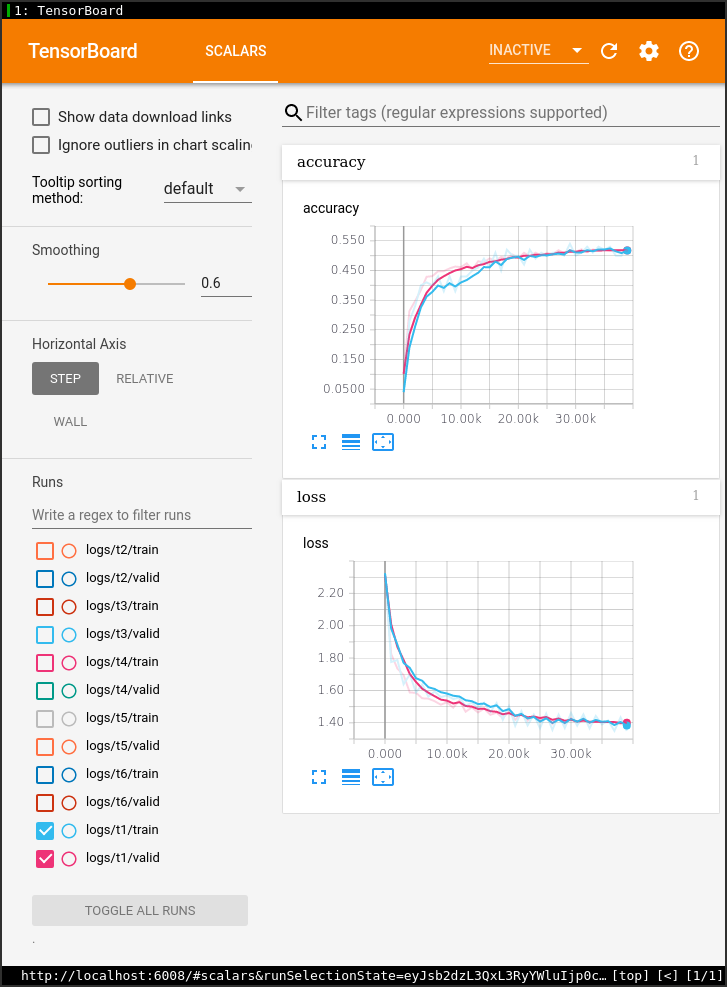
\includegraphics[width=0.6 \textwidth]{figure/t1.png}
	\caption{Default configuration}
	\label{fig:t1}
\end{figure}
The default configuration with 3 hidden layers, 64 neurons per layer, and a learning rate of 0.001 consistently resulted in validation accuracy between 51\% and 52\%, and a testing accuracy in the same range.


\section*{Testing configurations}
We also trained the model with the following four sets of hyperparameters:

\subsection*{Configuration 2}
Training the model using 5 hidden layers, 128 neurons per layer, and a learning rate of 0.001 resulted in a very similar accuracy as the default configuration, around 52\% for both validation and testing.
\begin{figure}[H]
	\centering
	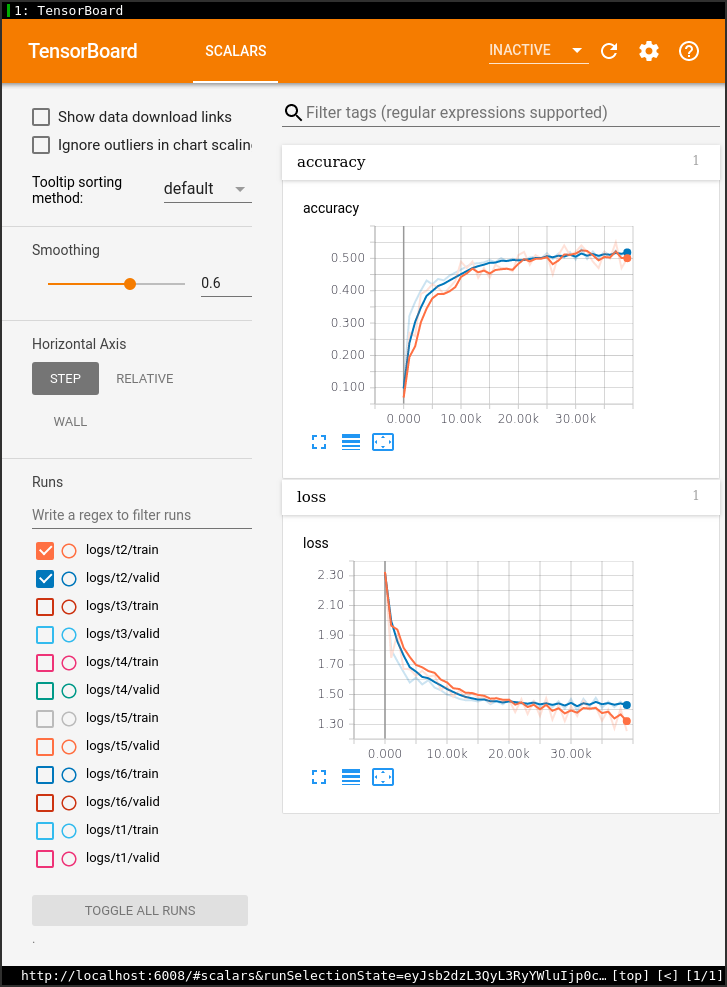
\includegraphics[width=0.6 \textwidth]{figure/t2.png}
	\caption{Configuration 2}
	\label{fig:t2}
\end{figure}

\subsection*{Configuration 3}
Training the model using the same learning rate and number of neurons as before but only one hidden layer again resulted in similar accuracy -- between 51\% and 52\%.
\begin{figure}[H]
	\centering
	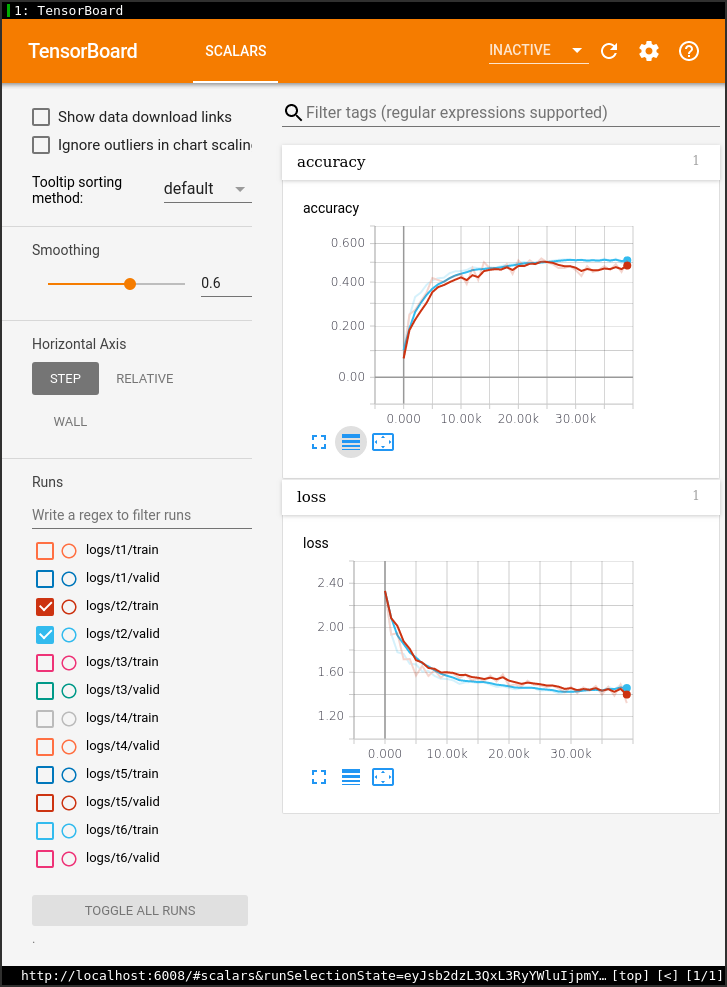
\includegraphics[width=0.6 \textwidth]{figure/t3.png}
	\caption{Configuration 3}
	\label{fig:t3}
\end{figure}

\subsection*{Configuration 4}
We saw that removing two layers had little no no effect on the accuracy, so we tried adding two layers, keeping the rest of the hyperparameters the same again.
This time, with five hidden layers, the model attained its highest accuracy yet, between 53\% and 54\% for validation and just over 53\% for testing.
\begin{figure}[H]
	\centering
	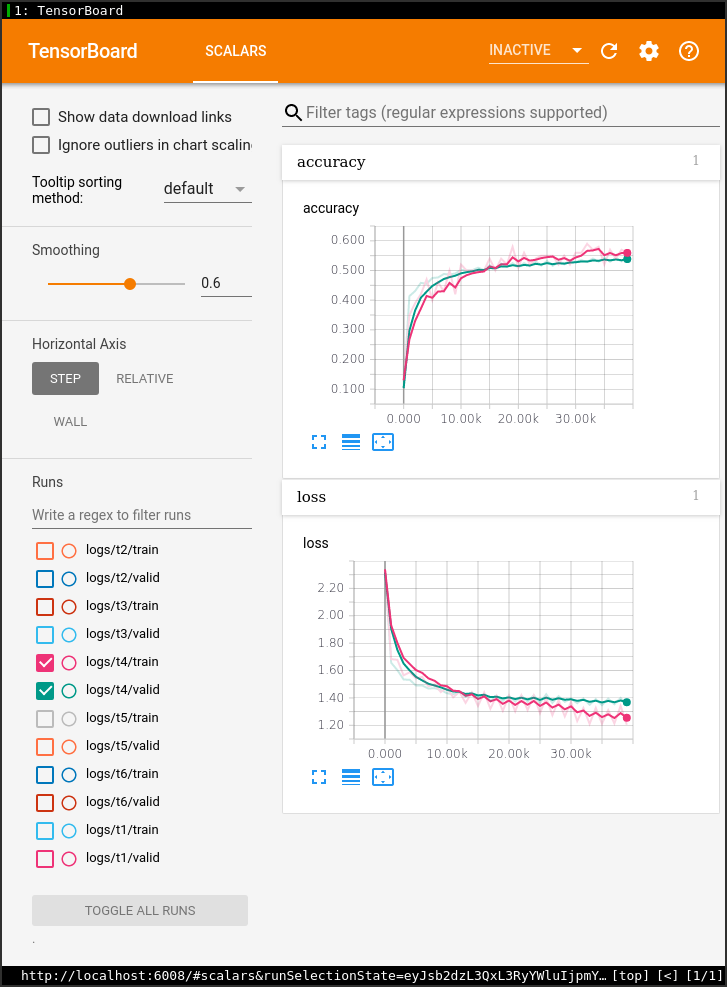
\includegraphics[width=0.6 \textwidth]{figure/t4.png}
	\caption{Configuration 4}
	\label{fig:t4}
\end{figure}

\subsection*{Configuration 5}
Our final experimental change to the architecture was quadrupling the number of neurons per hidden layer.
This change resulted in the highest accuracy we saw, just under 55\%.
\begin{figure}[H]
	\centering
	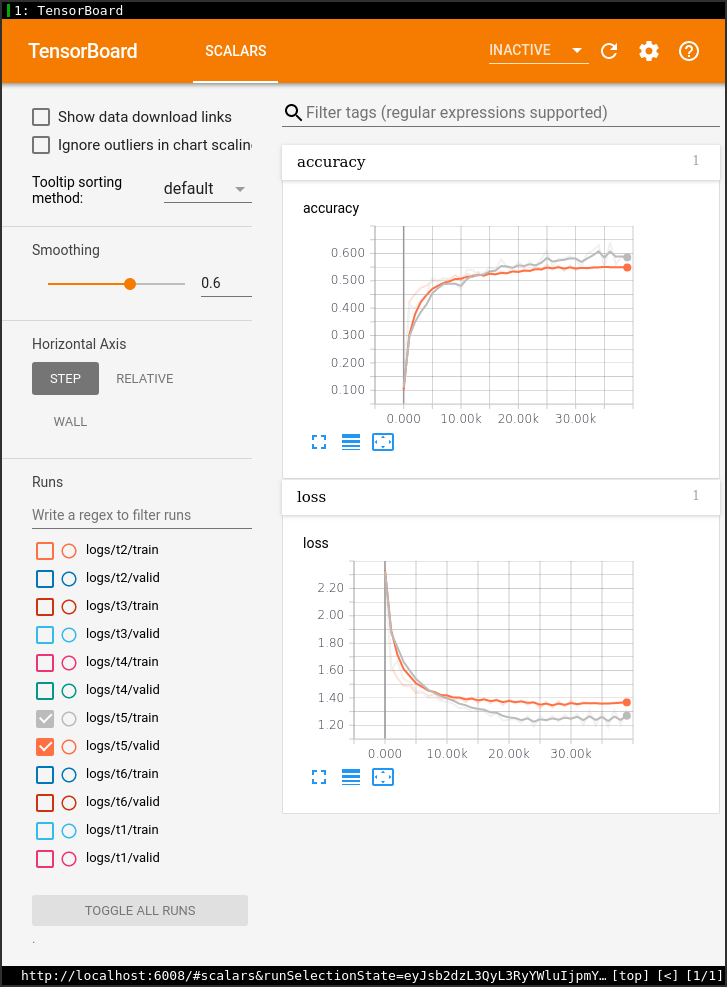
\includegraphics[width=0.6 \textwidth]{figure/t5.png}
	\caption{Configuration 5}
	\label{fig:t5}
\end{figure}

\subsection*{Configuration 6}
The final two tests were to see how changing the learning rate would affect the model's training.
The first test used the same hyperparameters as the default configuration, but used a learning rate of 0.0001 instead of 0.001.
This test resulted in training and validation accuracies of around 47\%-49\%, quite significantly
lower than our earlier experiments.
\begin{figure}[H]
	\centering
	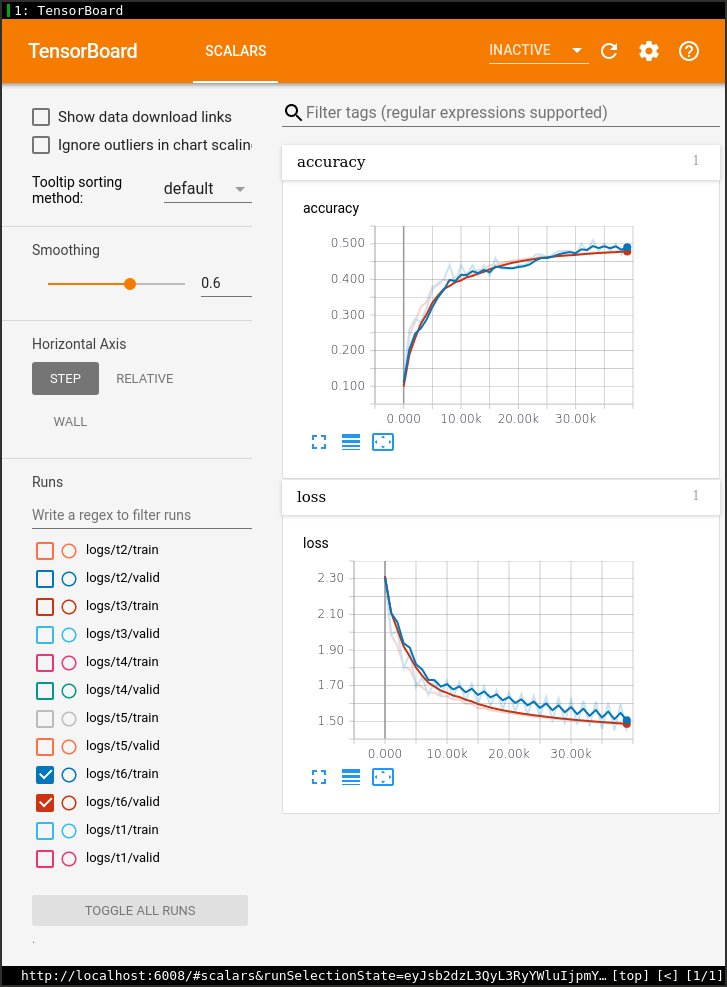
\includegraphics[width=0.6 \textwidth]{figure/t6.png}
	\caption{Configuration 6}
	\label{fig:t6}
\end{figure}

\subsection*{Configuration 7}
After the relative failure of our prior test, we decided to try increasing the learning rate significantly, up to 0.01.
This produced worse results -- around 38\%-40\% validation accuracy, and testing accuracy just above 39\%.
\begin{figure}[H]
	\centering
	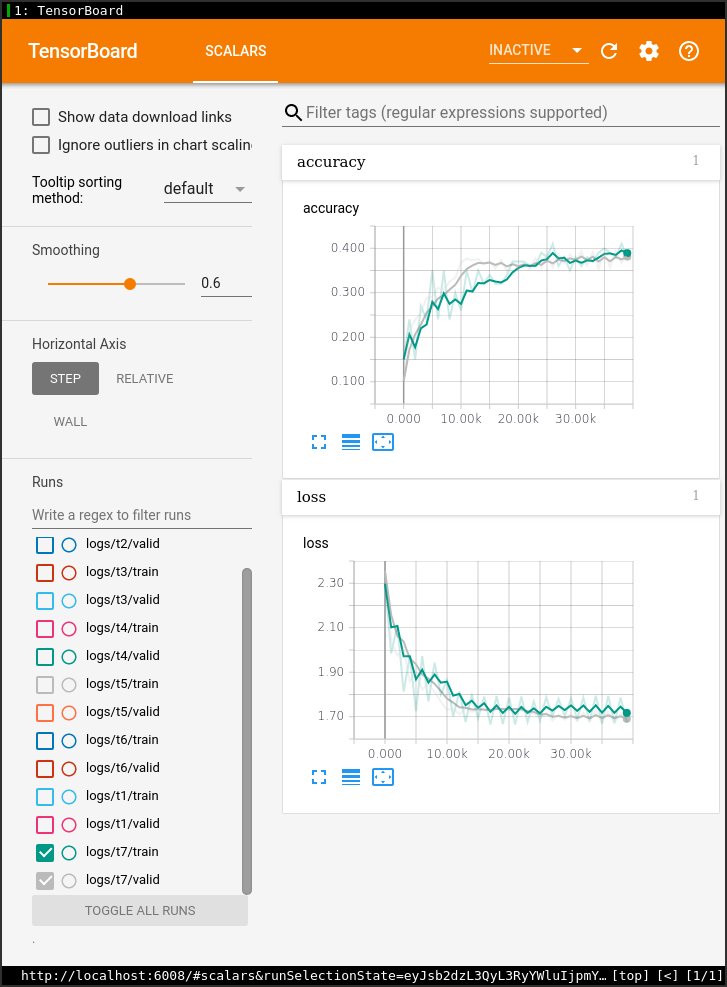
\includegraphics[width=0.6 \textwidth]{figure/t7.png}
	\caption{Configuration 7}
	\label{fig:t7}
\end{figure}

In all, we observed that modifying the learning rate drastically from the default of 0.001 resulted in a significant decrease in accuracy.
The main hyperparameters we were able to adjust to increase accuracy were the number of hidden layers and the number of neurons per hidden layer.
During our testsing, adding a small number of hidden layers or a large number of neurons to each hidden layer provided the greatest increase in model accuracy.


\end{document}
